\begin{comment}
TODO
\begin{itemize}
	\item all group fairness metrics
	\item vary sample size  and dimension of features (add statistics for each dataset in the figure)
	\item runtime vs max-order $ \lambda $
	\item draw $ 1/n $, $ 1/n^{1/2} $, $ 1/n^{1/3} $, std.
	\item \red{Experiment of fairness enhancing and attack algo on the same dataset.} 
\end{itemize}
\end{comment}





\clearpage


\begin{figure}
	\centering
	\subfloat[]{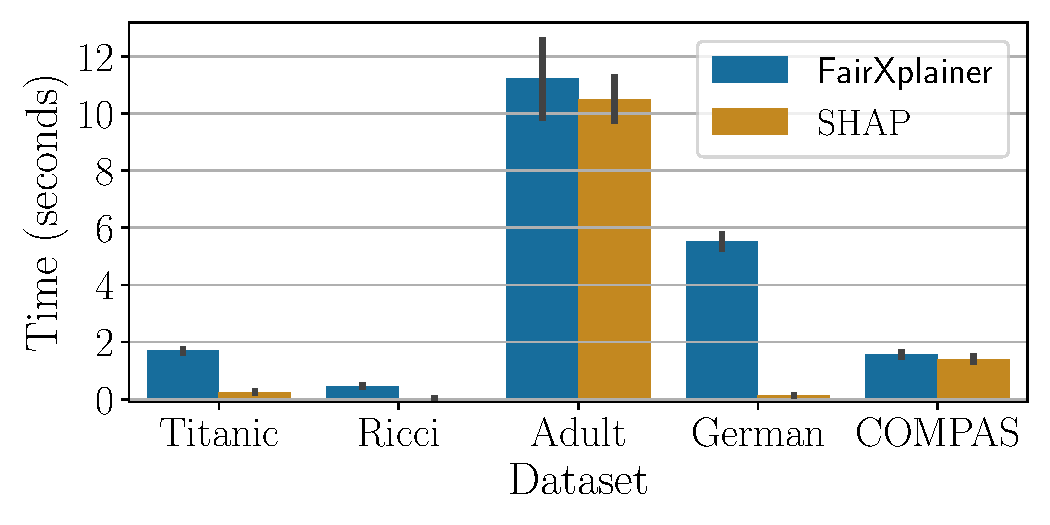
\includegraphics[scale=0.3]{figures/sp_train_time}}
	\subfloat[]{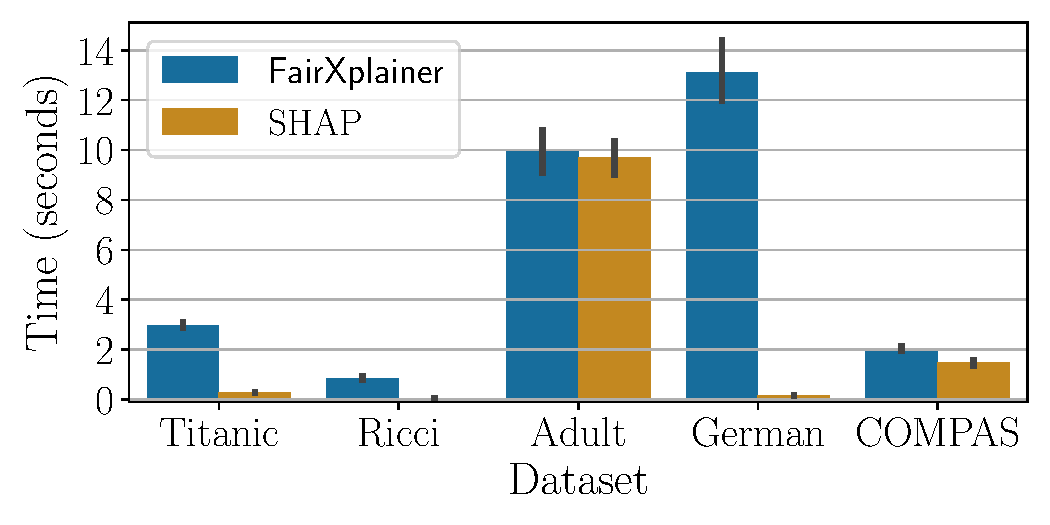
\includegraphics[scale=0.3]{figures/eo_train_time}}
	\subfloat[]{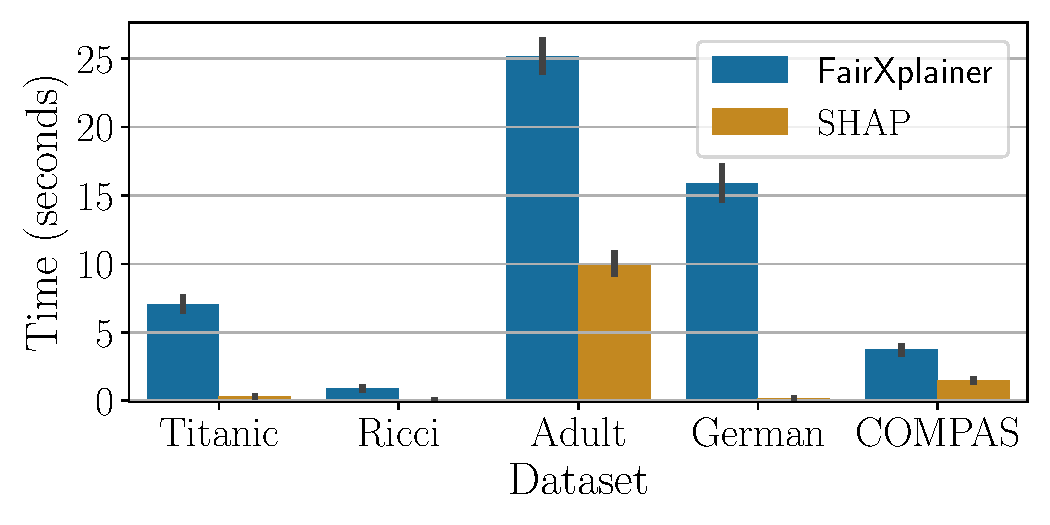
\includegraphics[scale=0.3]{figures/suff_train_time}}\\
	\subfloat[]{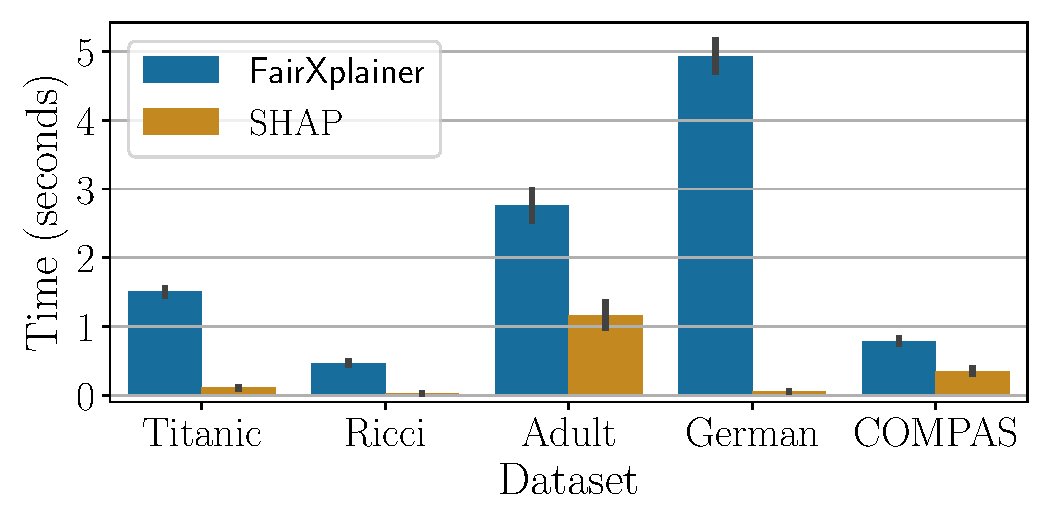
\includegraphics[scale=0.3]{figures/sp_test_time}}
	\subfloat[]{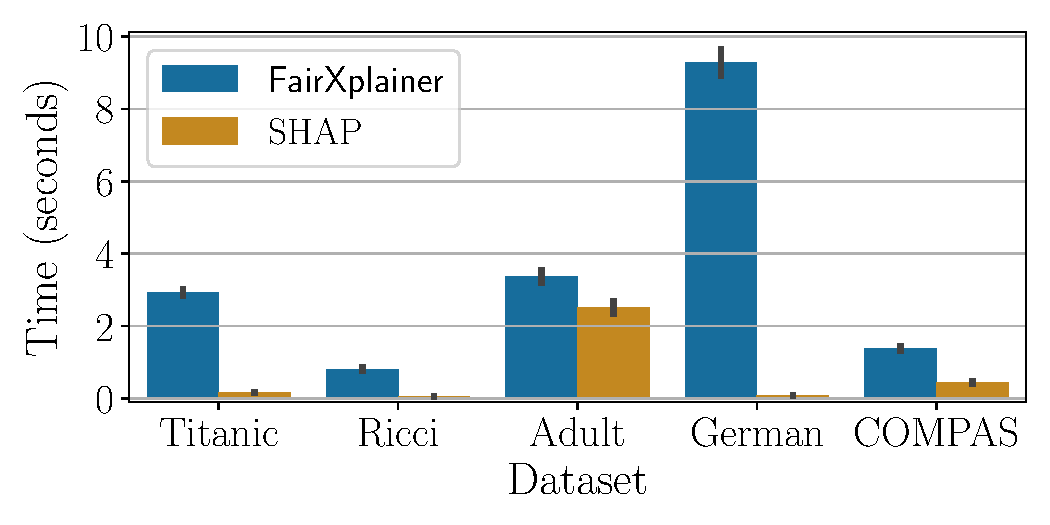
\includegraphics[scale=0.3]{figures/eo_test_time}}
	\subfloat[]{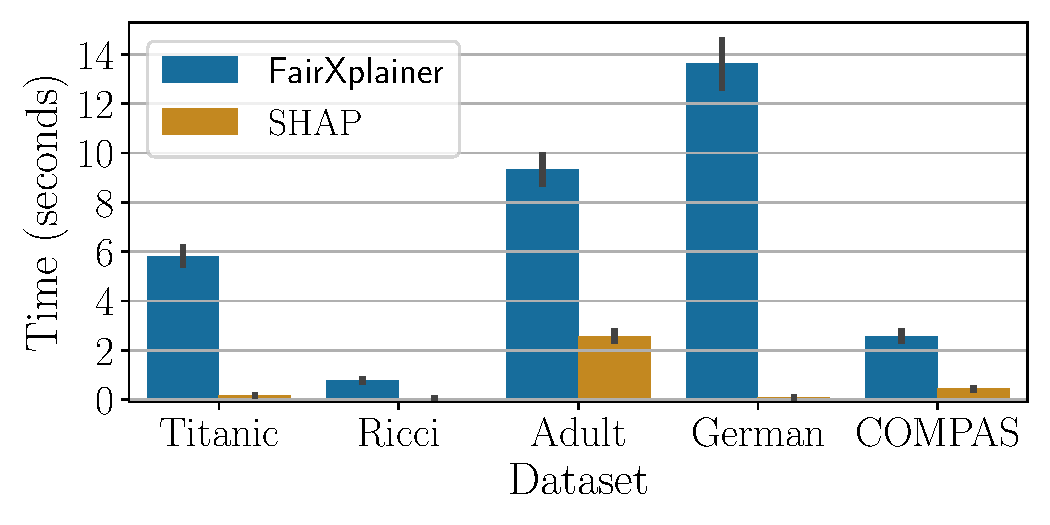
\includegraphics[scale=0.3]{figures/suff_test_time}}\\
	\caption{Comparison between {\framework} and SHAP on runtime. Lower values on the $ Y $-axis are better. \red{[Should be discussed in the Supplementary material.]}}
\end{figure}





\begin{figure}
	\centering
	\subfloat[Unsorted weights]{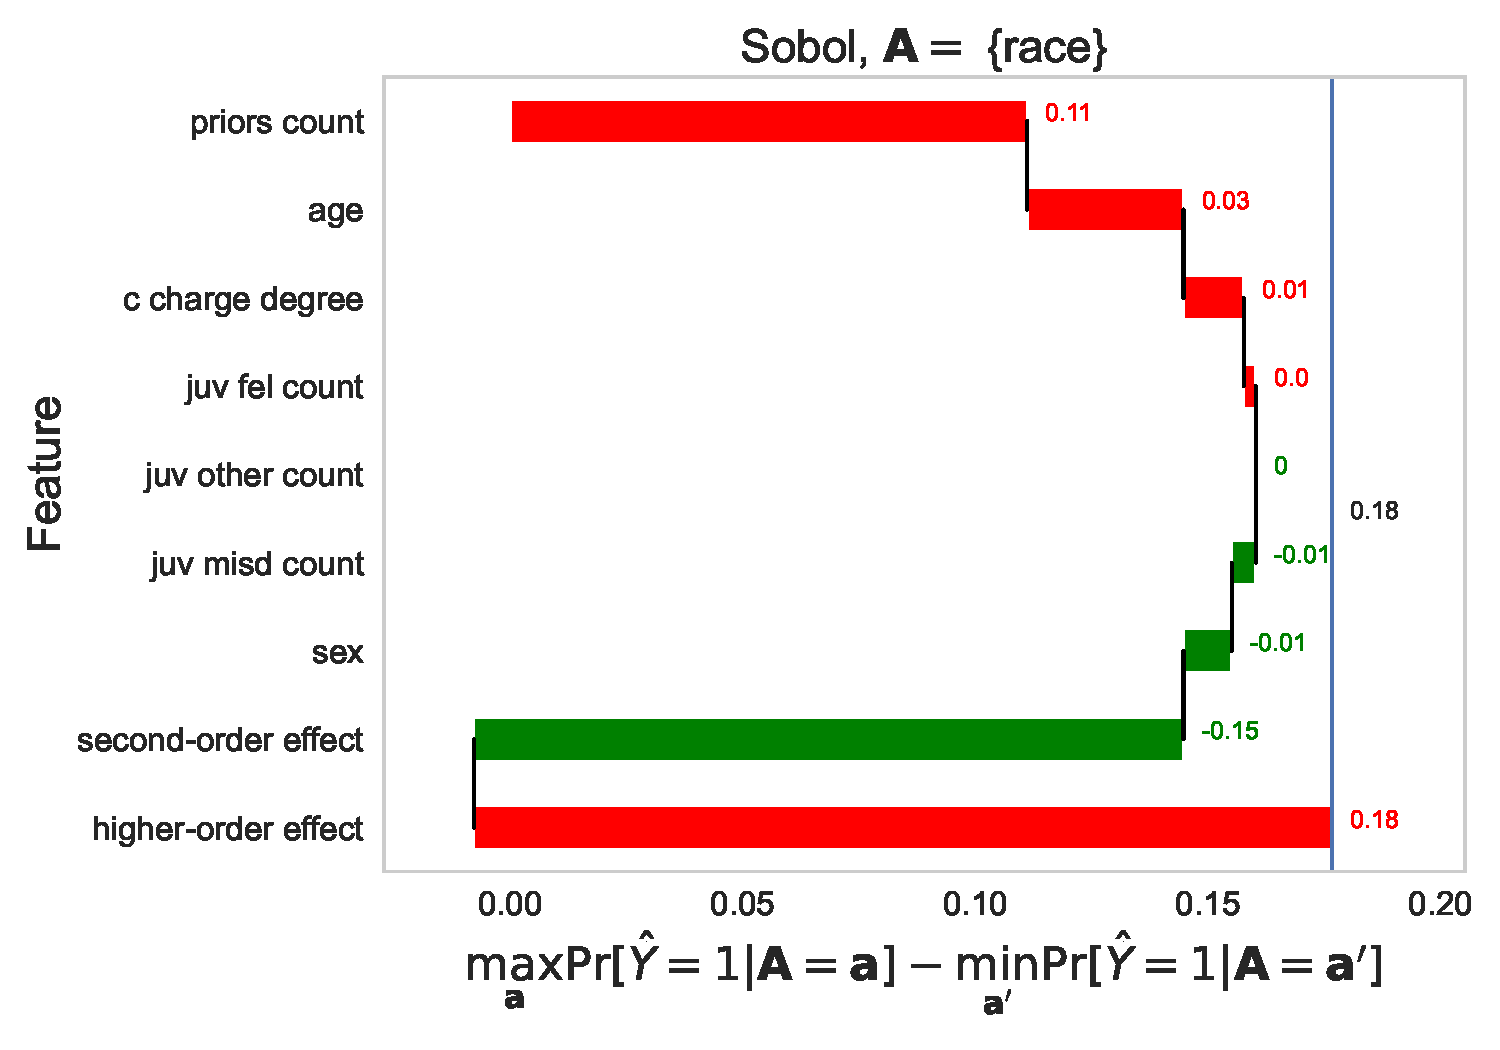
\includegraphics[scale=0.45]{figures/feature_weight_sobol_unsorted}}\\
	\subfloat[Sorted weights including first and second order effect]{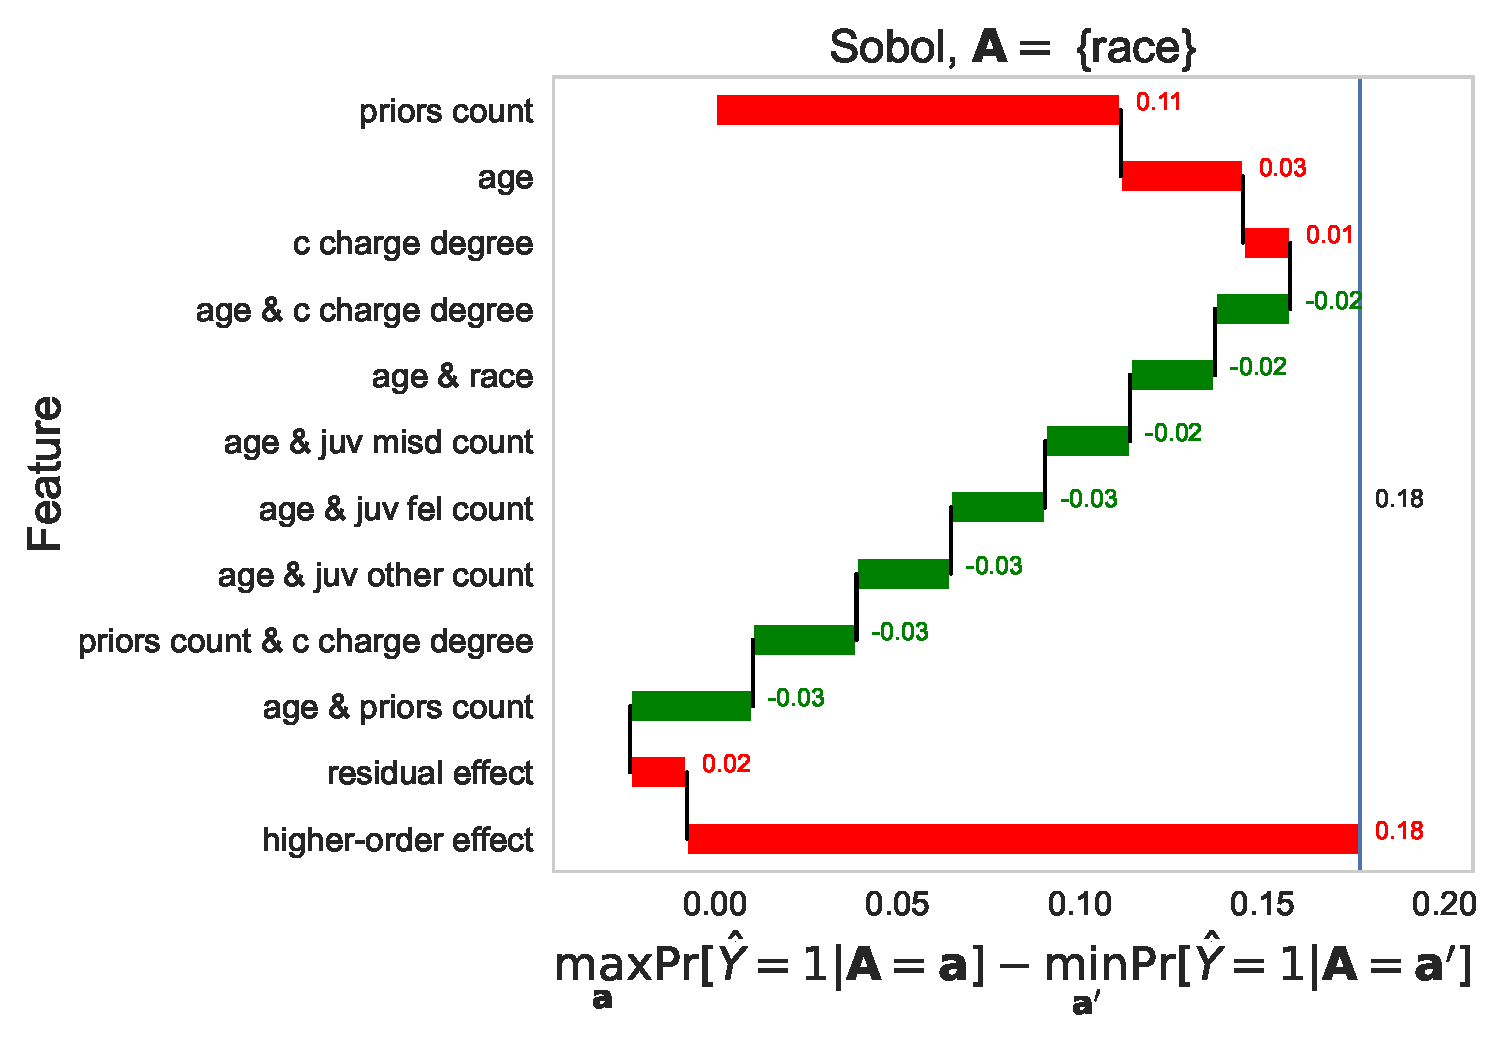
\includegraphics[scale=0.45]{figures/feature_weight_sobol}}\\
	\caption{Explaining statistical parity in COMPAS dataset for the sensitive feature `race' using Sobol method. This approach takes the (independent) distribution of features as input instead of a dataset. We apply KDE (Kernel Density Estimation) to learn the PDF of each feature.}
\end{figure}


\begin{figure}
	\centering
	\subfloat{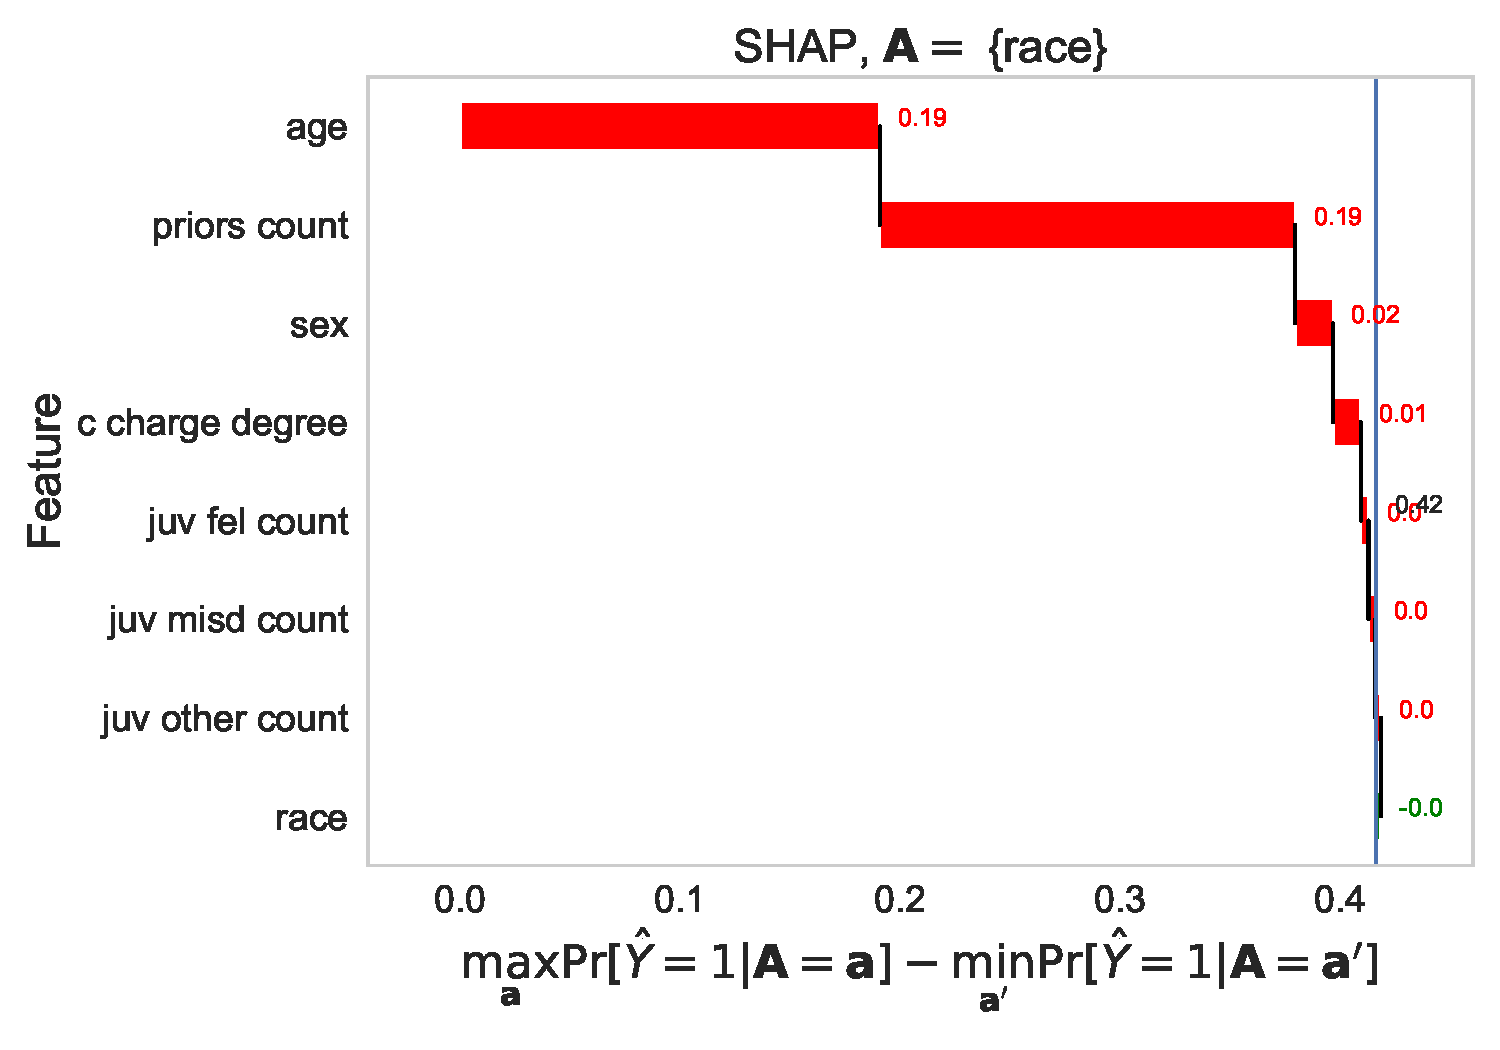
\includegraphics[scale=0.45]{figures/feature_weight_shap}}\\
	\caption{Explaining statistical parity in COMPAS dataset for the sensitive feature `race' using Shap method. This method is based on local explanations of classifiers. We observe higher discrepancy of this explanation as the computed statistical parity is often far from the exact value. Shap method can explain effect of individual features, which is a crucial limitation.}
\end{figure}

\begin{figure}
	\centering
	\subfloat{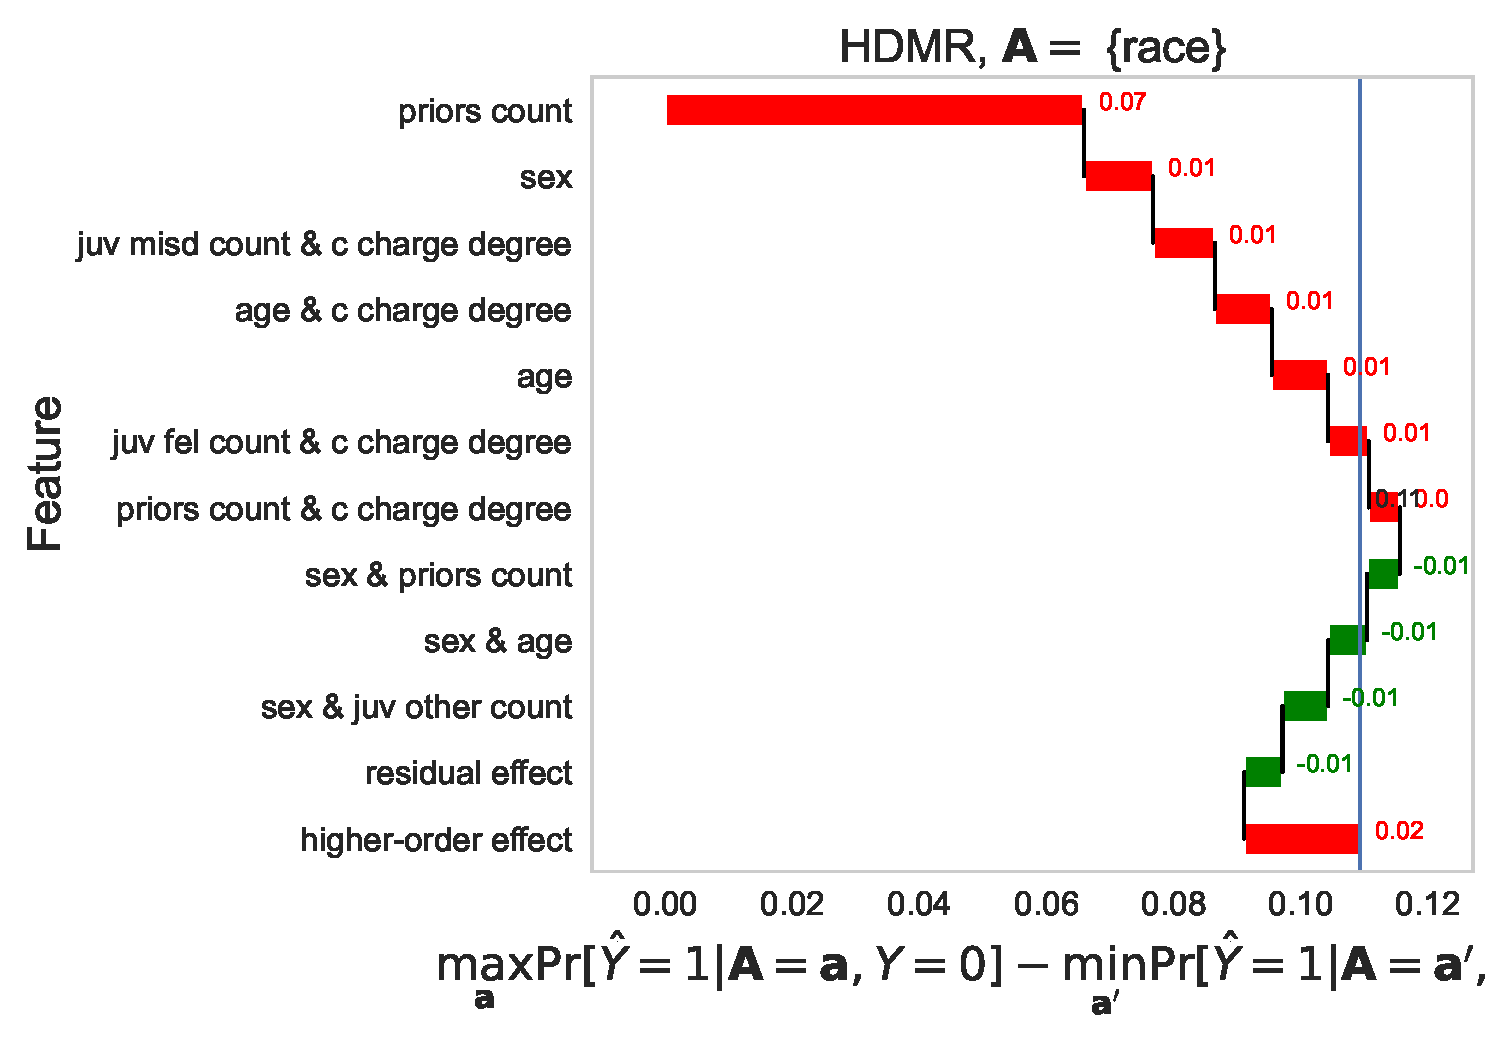
\includegraphics[scale=0.45]{figures/feature_weight_eo_y_0}}\\
	\subfloat{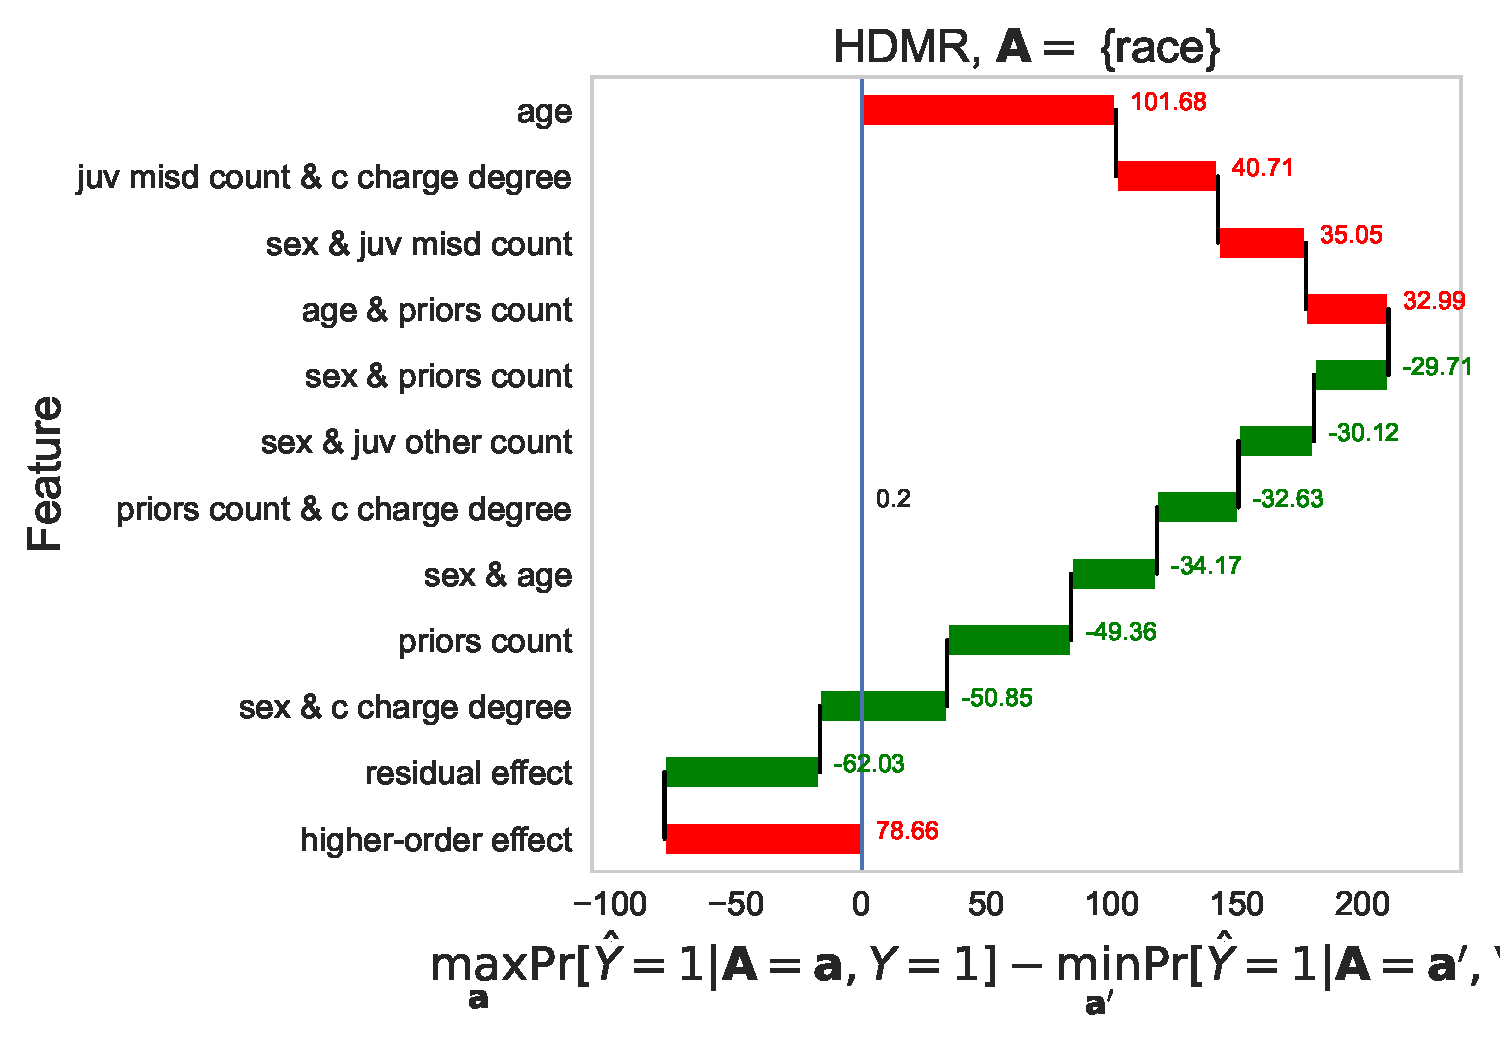
\includegraphics[scale=0.45]{figures/feature_weight_eo_y_1}}\\
	\caption{Explaining equalized odds in COMPAS dataset for the sensitive feature `race' using HDMR method.}
\end{figure}


\begin{figure}
	\centering
	\subfloat{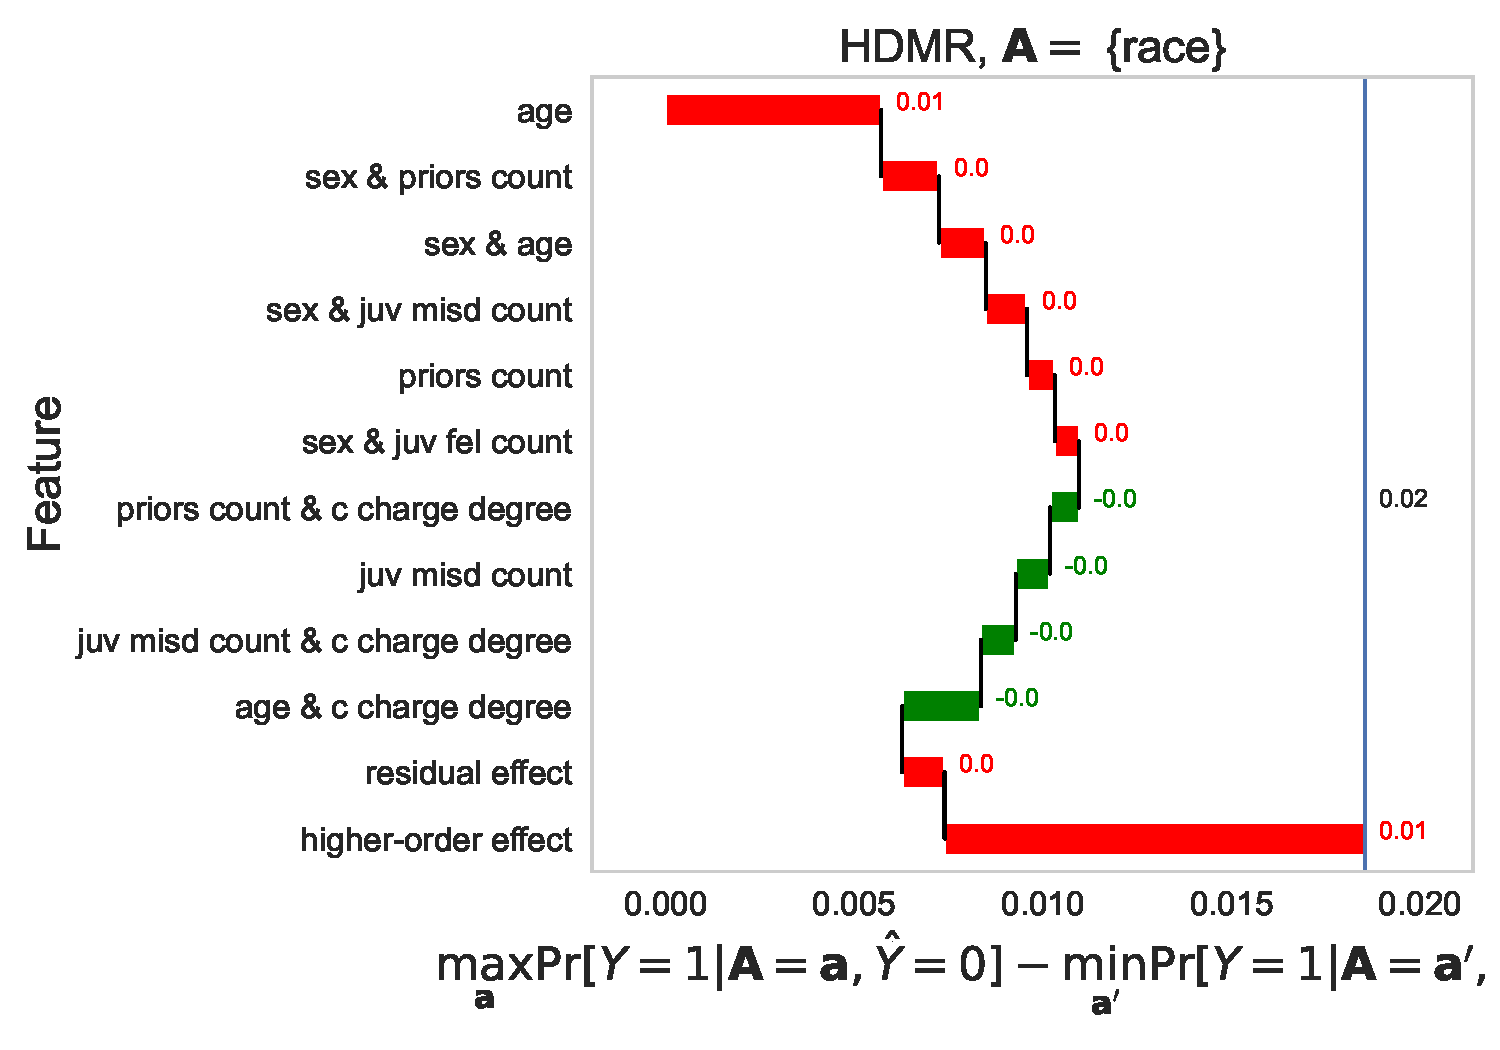
\includegraphics[scale=0.45]{figures/feature_weight_sufficiency_y_0}}\\
	\subfloat{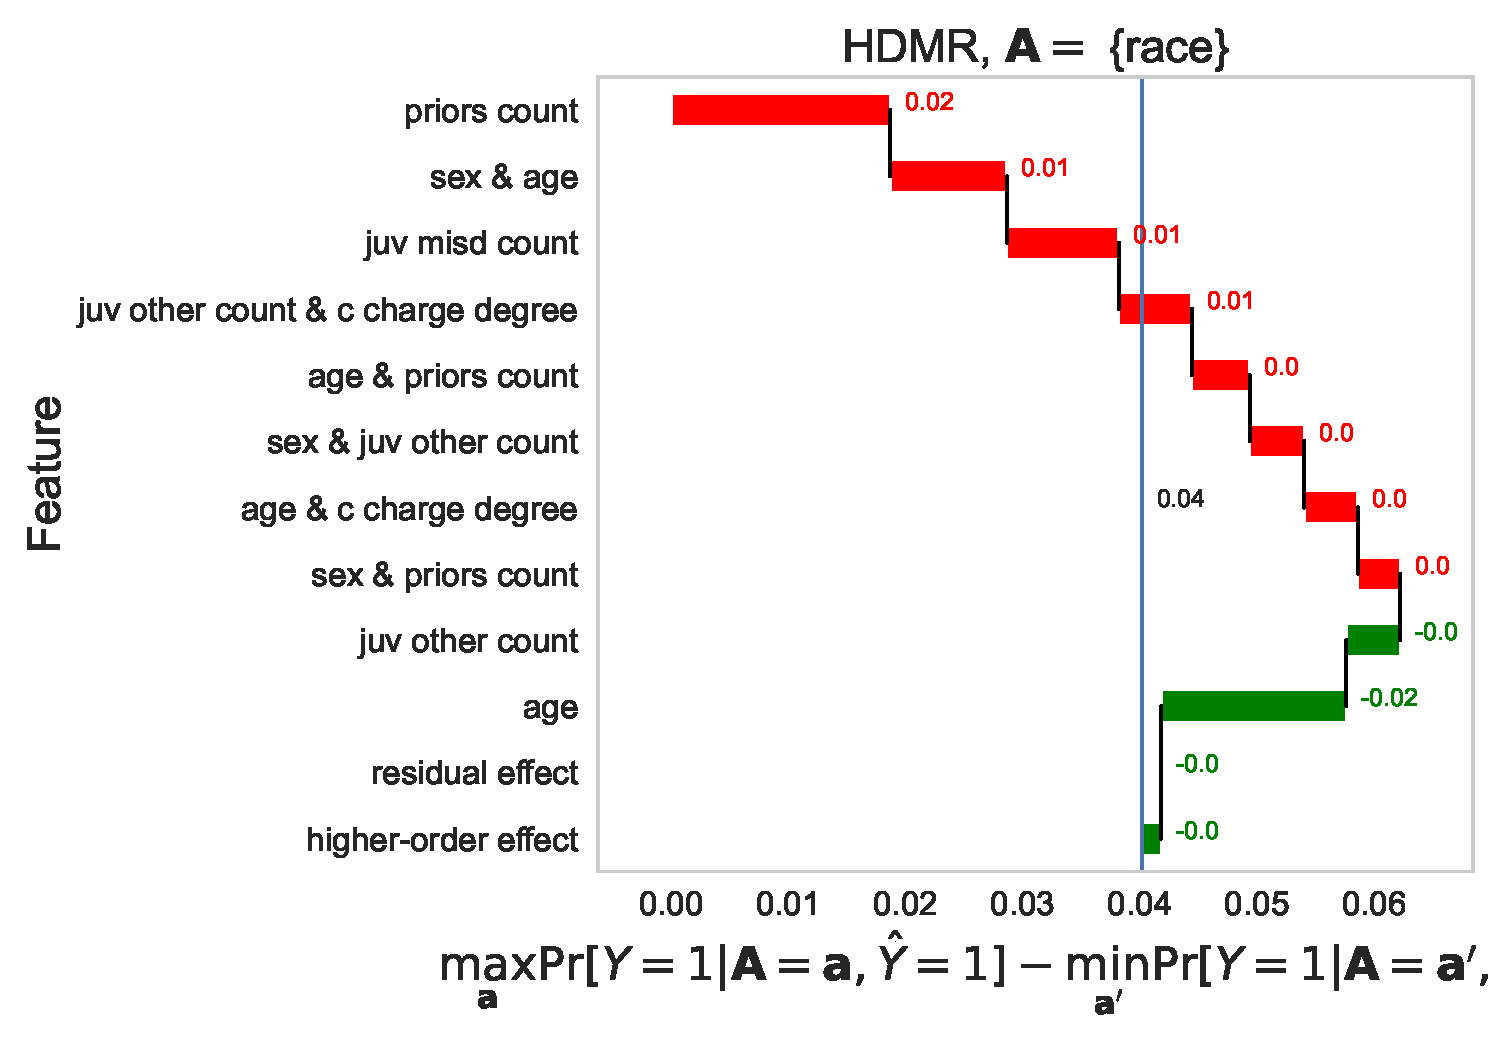
\includegraphics[scale=0.45]{figures/feature_weight_sufficiency_y_1}}\\
	\caption{Explaining sufficiency fairness metrics in COMPAS dataset for the sensitive feature `race' using HDMR method.}
\end{figure}


\begin{figure}
	\centering
	\subfloat{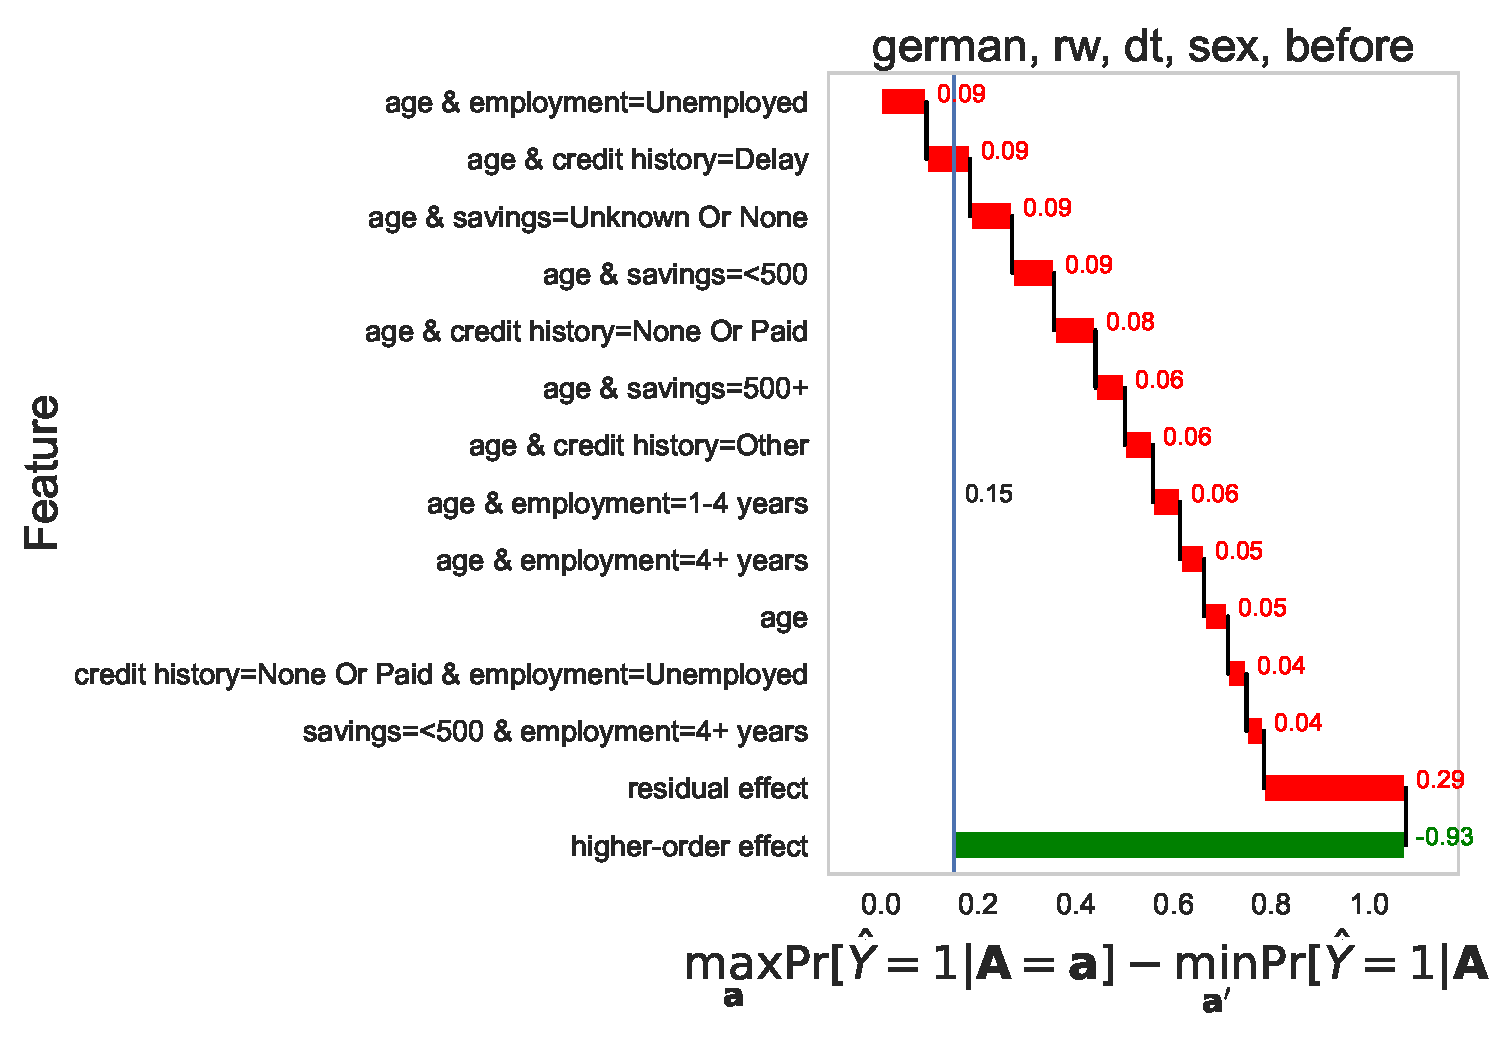
\includegraphics[scale=0.45]{figures/german_rw_dt_sex_before}}\\
	\subfloat{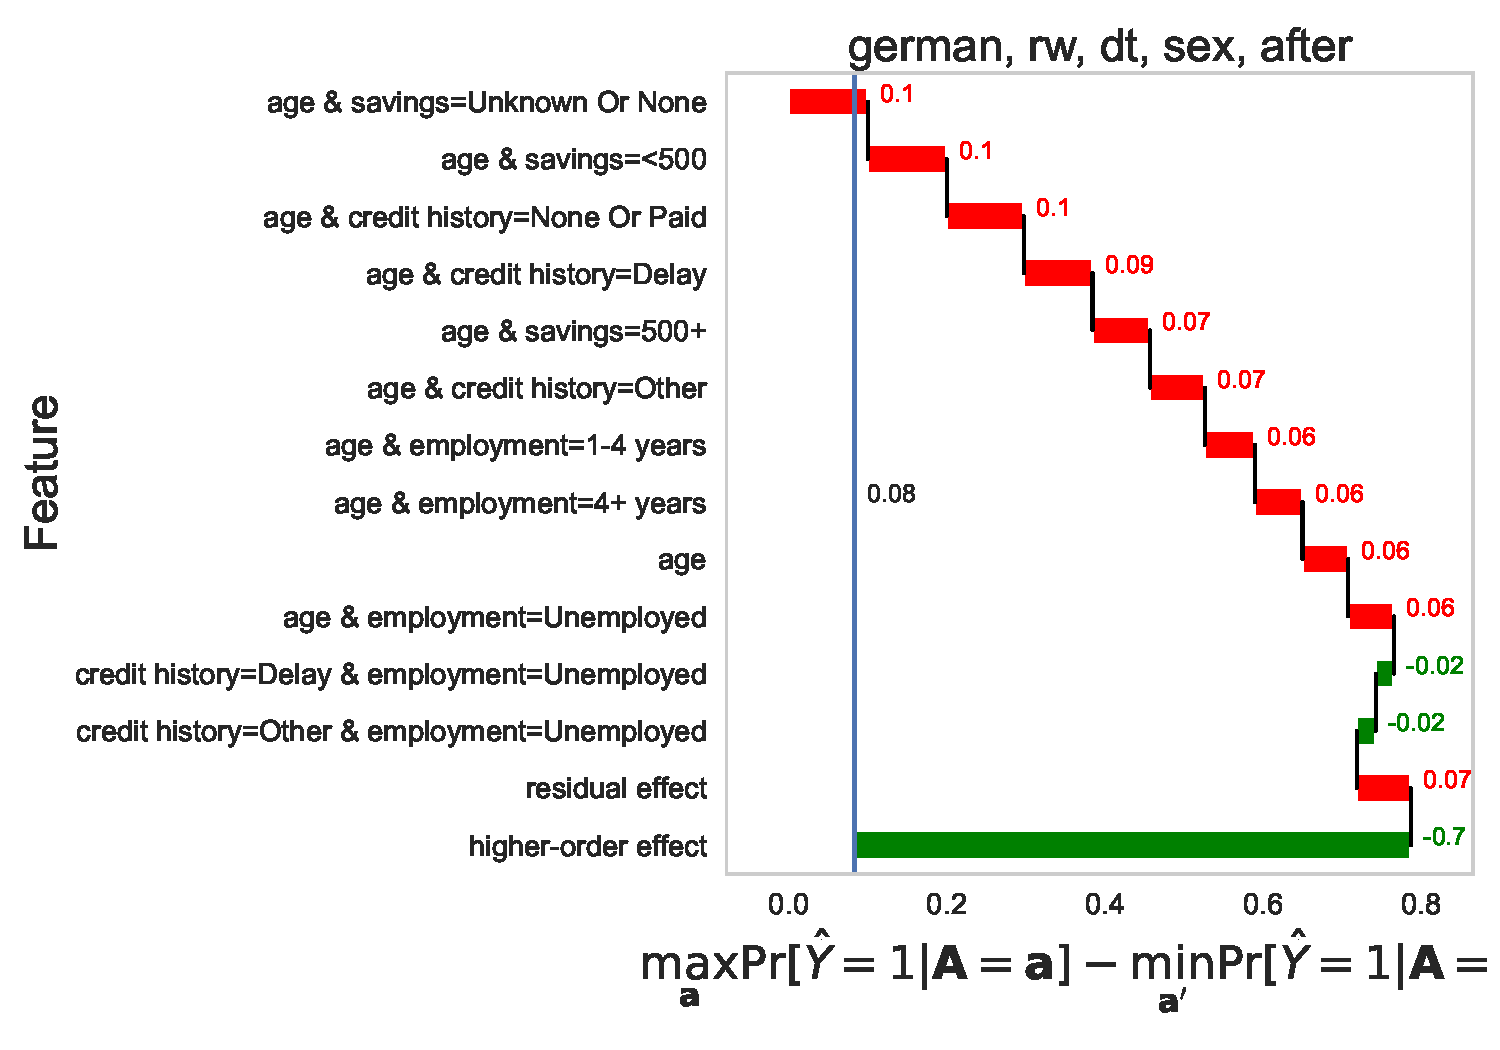
\includegraphics[scale=0.45]{figures/german_rw_dt_sex_after}}
	\caption{Fairness enhancing preprocessing algorithm, reweighing..}
\end{figure}

\begin{figure}
	\centering
	\subfloat{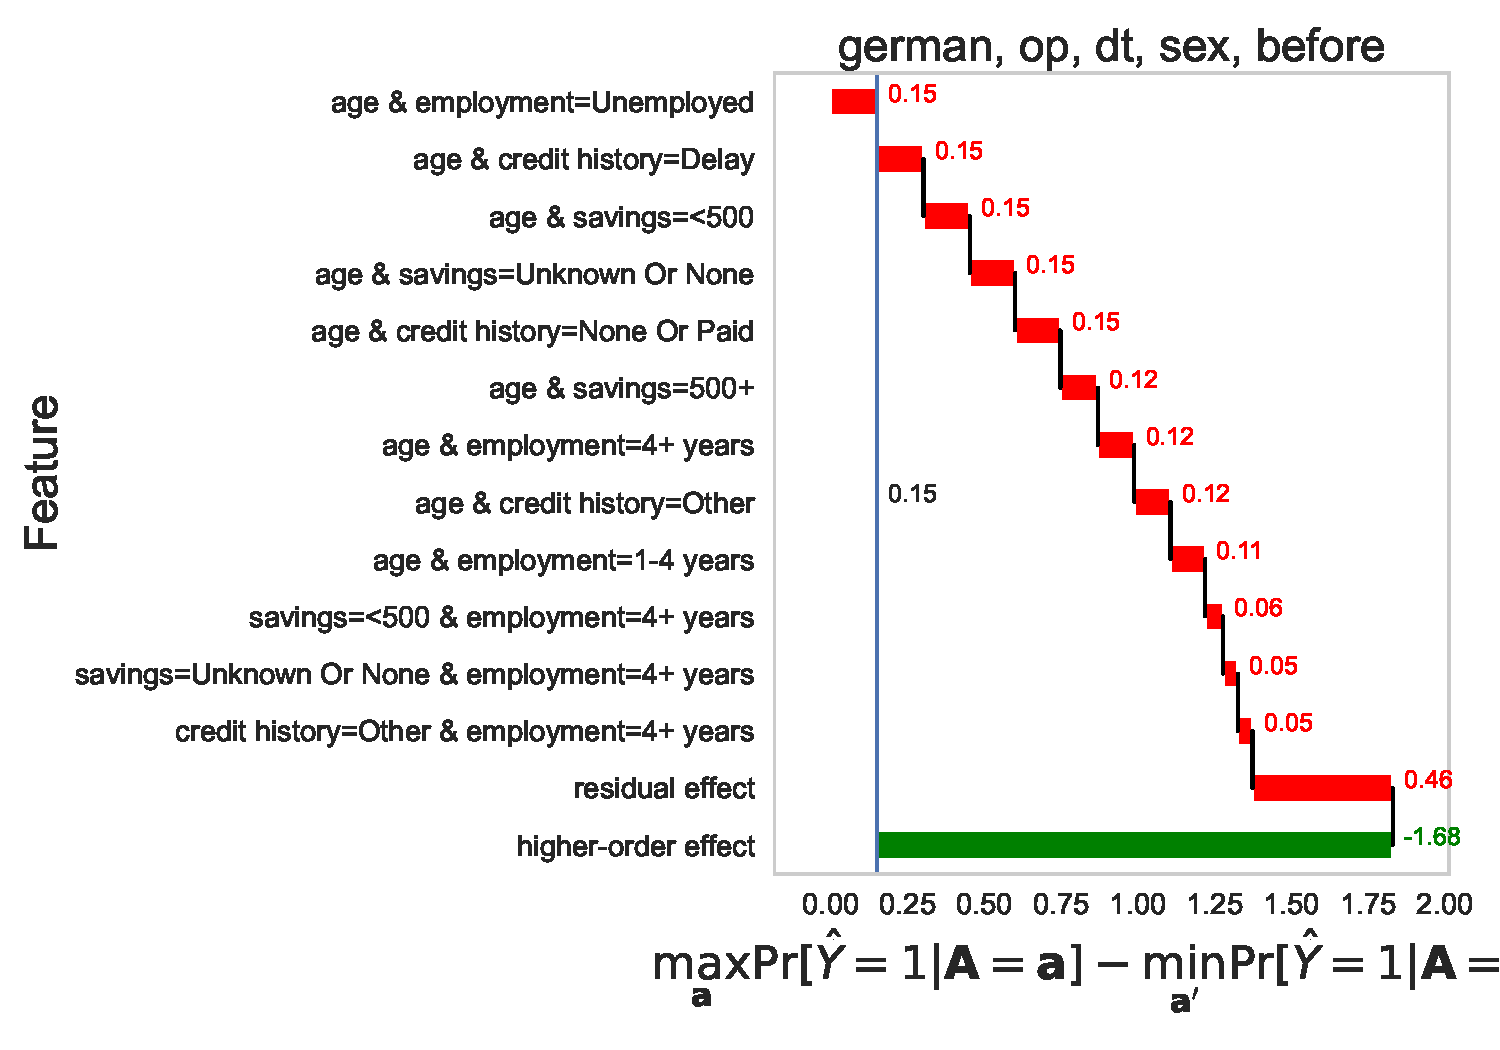
\includegraphics[scale=0.45]{figures/german_op_dt_sex_before}}\\
	\subfloat{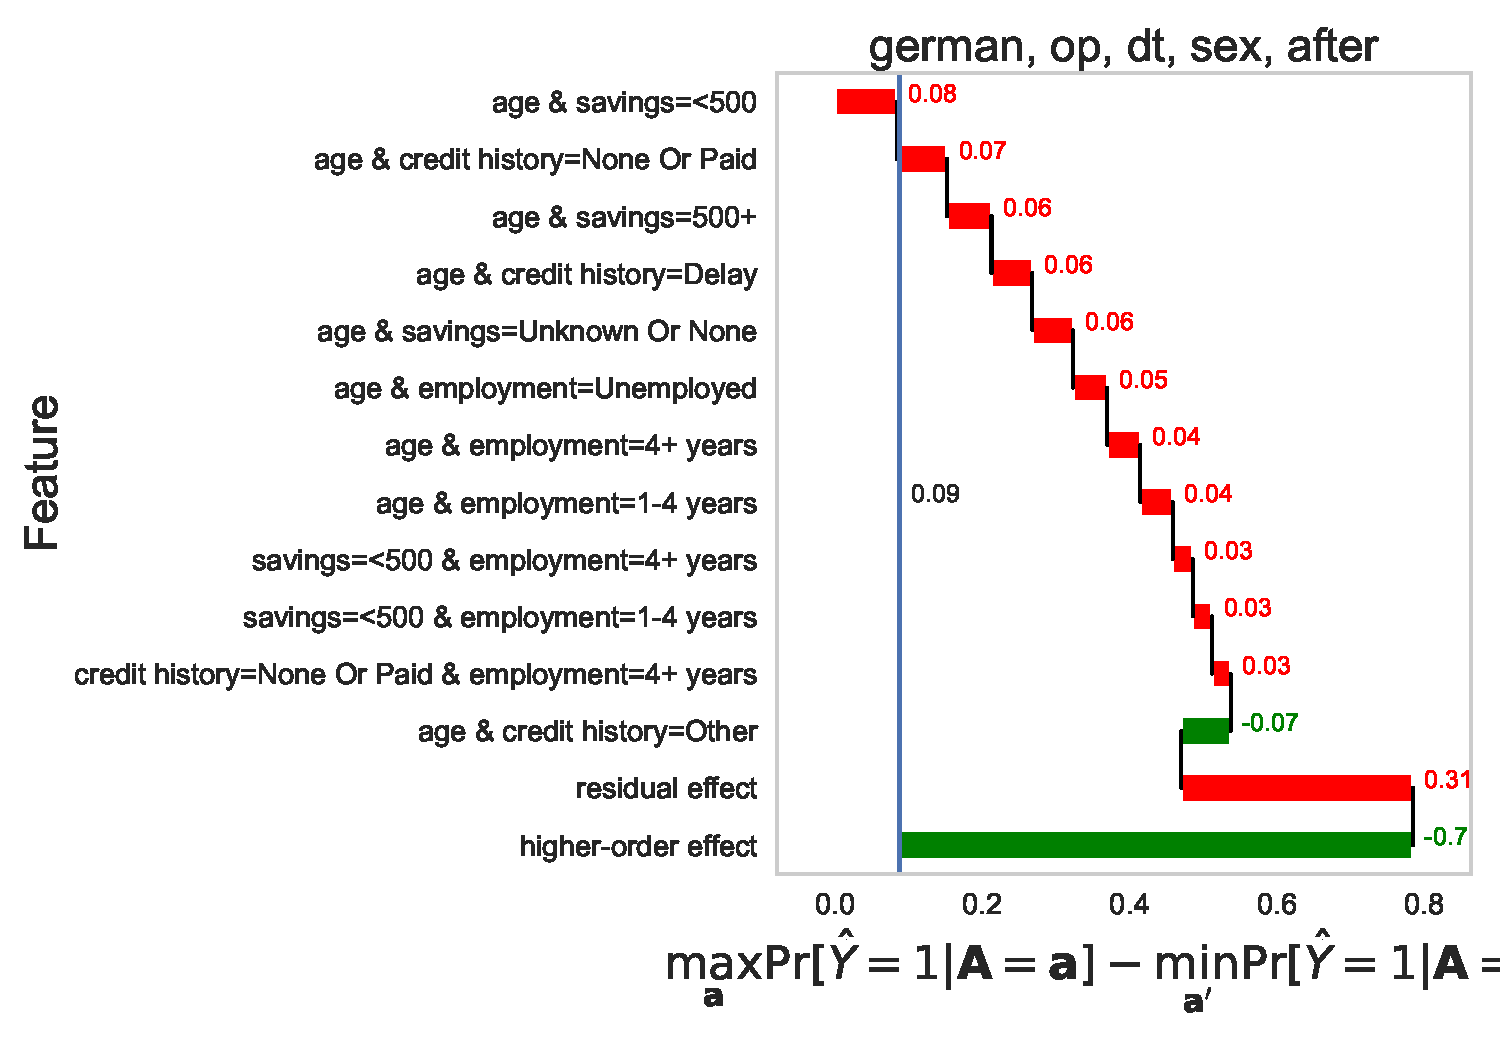
\includegraphics[scale=0.45]{figures/german_op_dt_sex_after}}
	\caption{Fairness enhancing preprocessing algorithm, optimized preprocessing. f\red{X axis should have the same X limit}}
\end{figure}


\begin{figure}
	\centering
	\subfloat{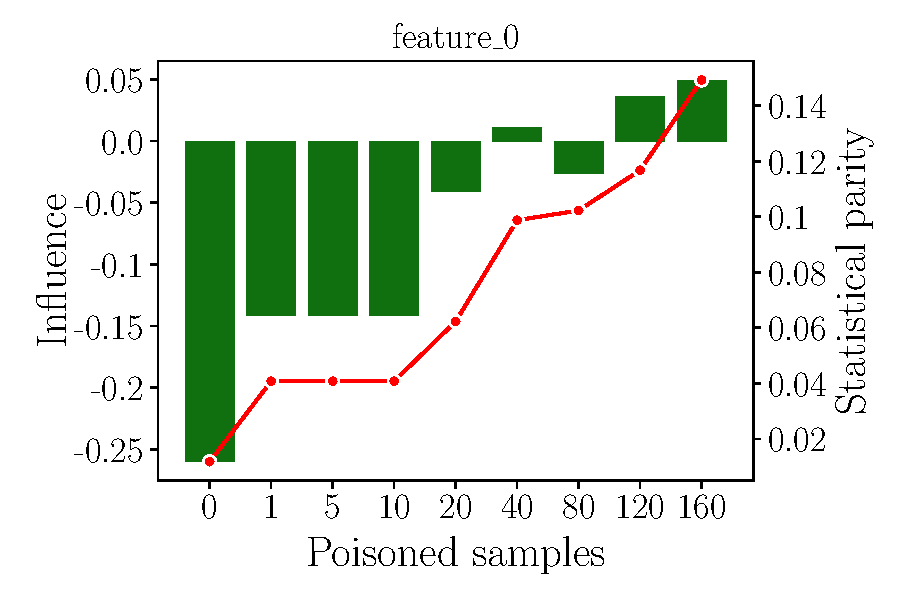
\includegraphics[scale=0.45]{figures/fairness_attack_feature_0}}
	\subfloat{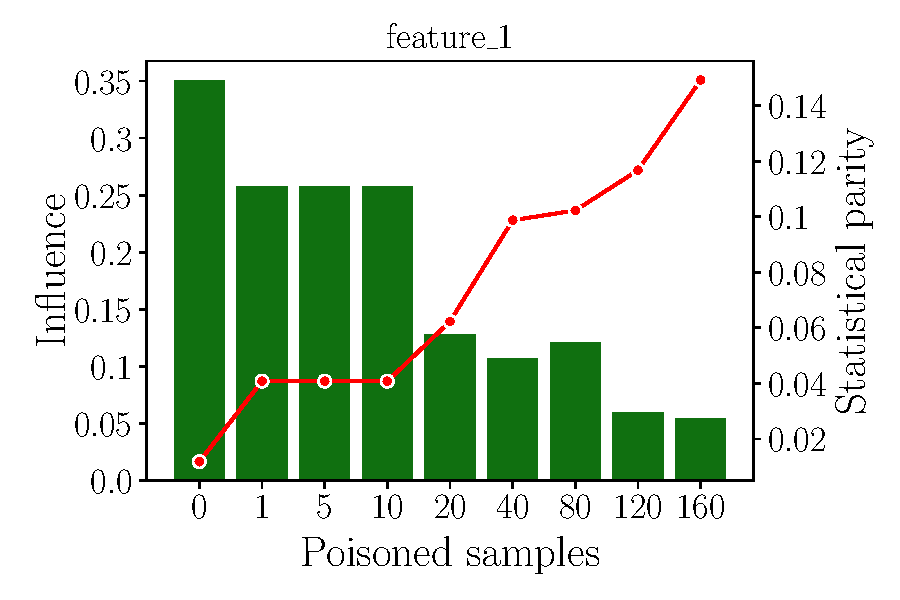
\includegraphics[scale=0.45]{figures/fairness_attack_feature_1}}\\
	\subfloat{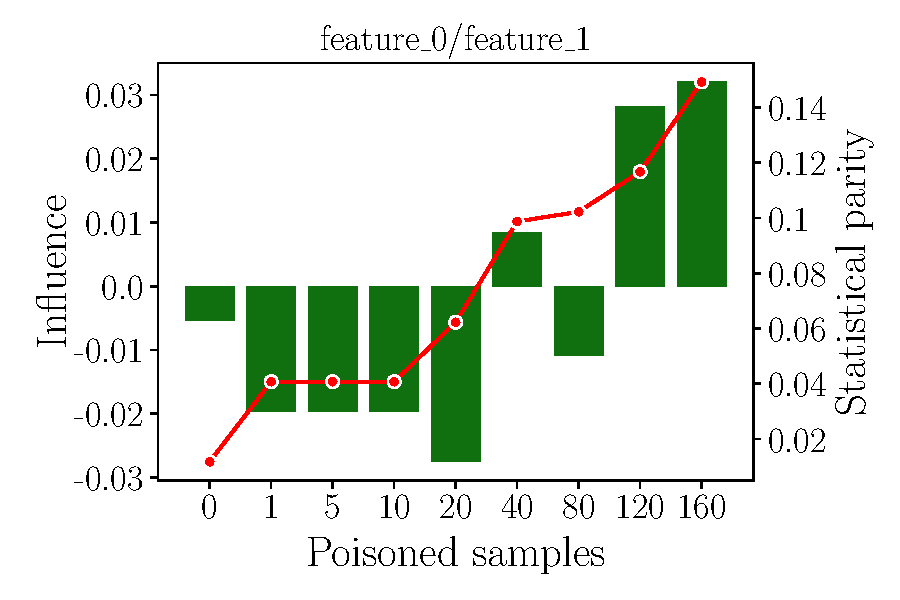
\includegraphics[scale=0.45]{figures/fairness_attack_feature_0_and_feature_1}}
	\subfloat{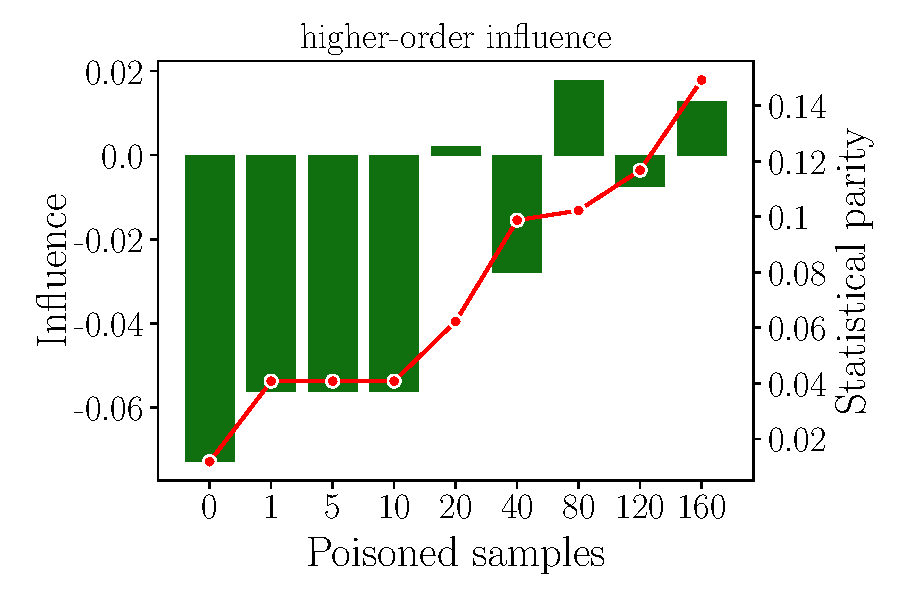
\includegraphics[scale=0.45]{figures/fairness_attack_higher-order_influence}}\\
	\caption{Fairness attack. Fairness influence is presented  in bar while statistical parity is shown in a line.}
\end{figure}


